\documentclass[12pt]{article}
\usepackage{tikz}
\usepackage{float}
\usepackage{chngpage}
\begin{document}
\title{Computer Science 118, Homework 1}
\date{October 18th, 2018}
\author{Michael Wu\\UID: 404751542}
\maketitle

\section*{Problem 1}

\paragraph{a)}

There are 3 periods of the signal. This makes sense because the first harmonic frequency is \(1000\) Hz.

\paragraph{b)}

The plots of the first three harmonics are shown below.
\begin{figure}[H]
    \begin{adjustwidth}{-2in}{-2in}
        \begin{center}
            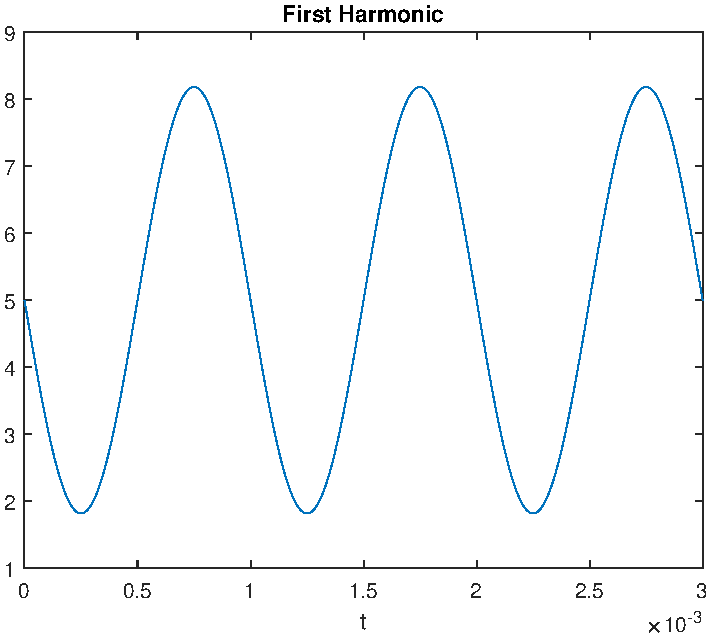
\includegraphics[width=2in]{problem1-first.pdf}
            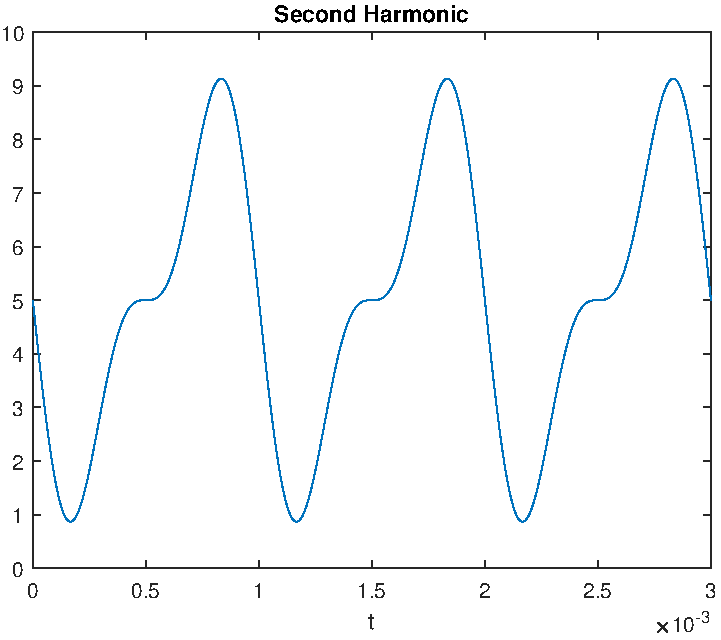
\includegraphics[width=2in]{problem1-second.pdf}
            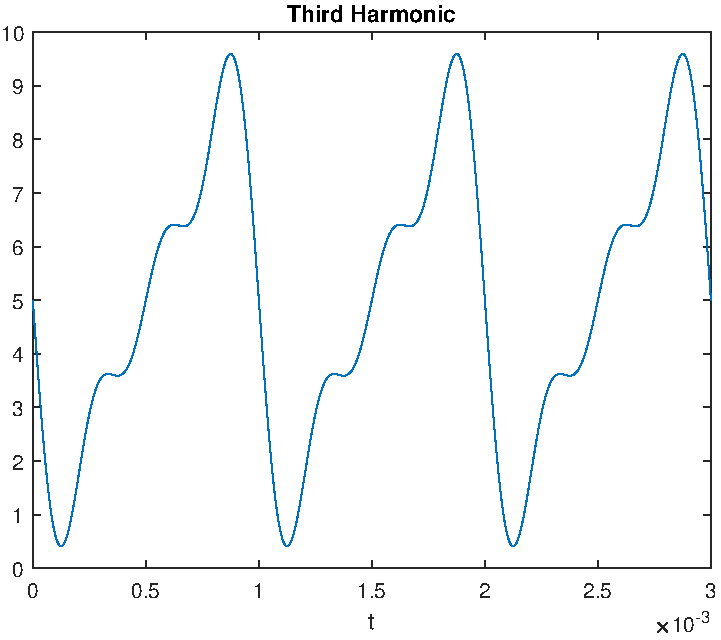
\includegraphics[width=2in]{problem1-third.pdf}
        \end{center}
    \end{adjustwidth}
\end{figure}

\paragraph{c)}

It appears to be a sawtooth wave with a frequency of \(1000\) Hz, a minimum of 0, and a maximum of 10.

\paragraph{d)}

Assuming that this is baseband bandwidth, only the first harmonic would be allowed to go through, so the output
signal would look like the first harmonic.

\section*{Problem 2}

\paragraph{a)}

The receiver will measure 0V, 4V, then 4V. Thus it will correctly receive the bits 011.
\begin{figure}[H]
    \begin{center}
        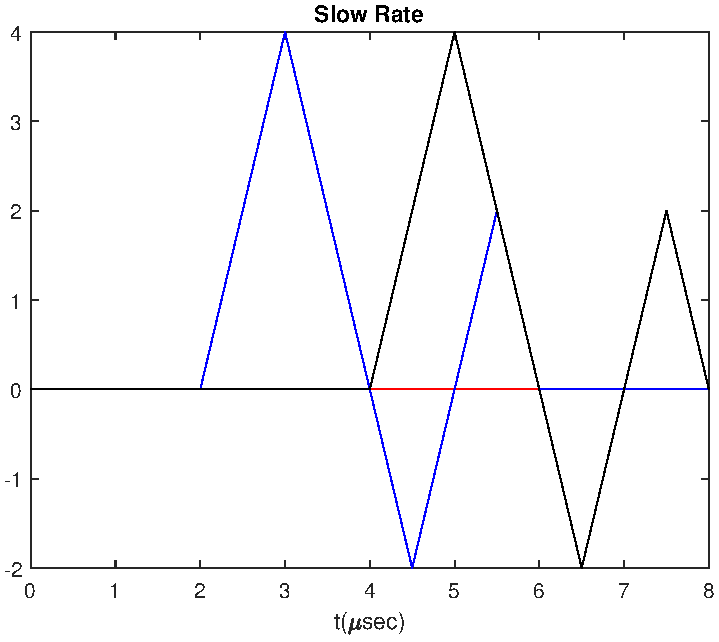
\includegraphics[width=2.5in]{problem2a.pdf}
    \end{center}
\end{figure}

\paragraph{b)}

The receiver will measure 0V, 4V, then 4V. Thus it will correctly receive the bits 011.
\begin{figure}[H]
    \begin{center}
        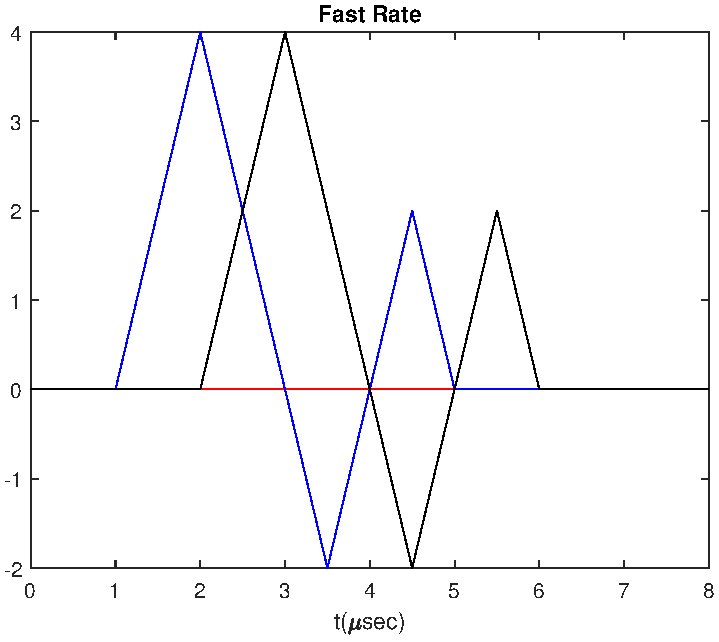
\includegraphics[width=2.5in]{problem2b.pdf}
    \end{center}
\end{figure}

\paragraph{c)}

The receiver will measure 2V, 6V, then 6V. Thus it will receive the bits 111. Therefore bit interference has caused the 0 to become a 1. Note that all the bits experience
bit interference, as the measured voltages are increased due to the effects of other bits.

\begin{figure}[H]
    \begin{center}
        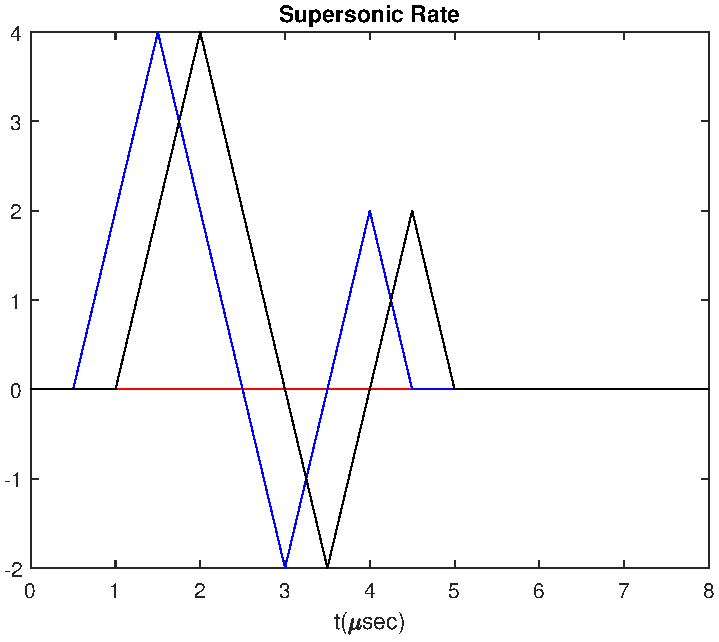
\includegraphics[width=2.5in]{problem2c.pdf}
    \end{center}
\end{figure}

\section*{Problem 3}

\paragraph{a)}

The waveform is shown in the following figure.
\begin{figure}[H]
    \begin{center}
        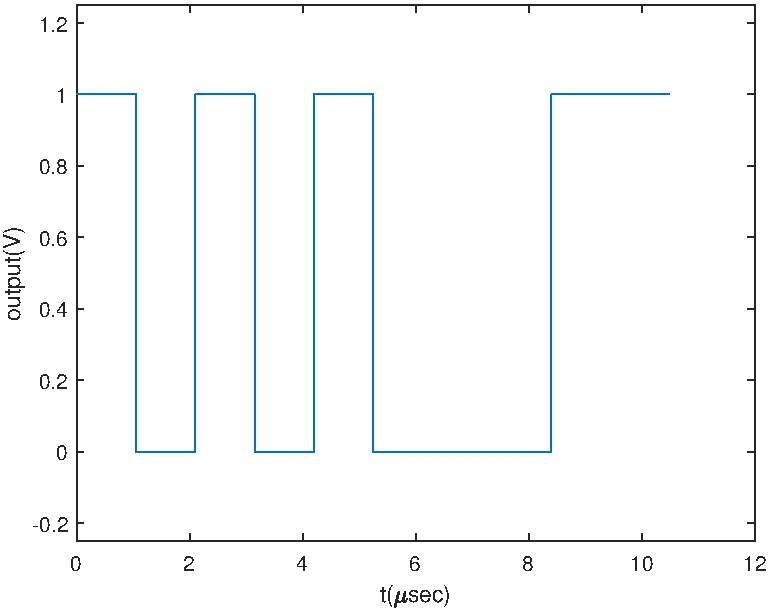
\includegraphics[width=2.5in]{problem3a.pdf}
    \end{center}
\end{figure}

\paragraph{b)}

The sampling will happen \(0.475\mu\)s earlier than it should have if there is no clock recovery.

\paragraph{c)}

With clock recovery, the sampling will happen at times \(0.5\mu\)s, \(1.5\mu\)s, \(2.55\mu\)s, \(3.60\mu\)s, \(4.65\mu\)s, \(5.70\mu\)s, \(6.75\mu\)s,
\(7.80\mu\)s, \(8.85\mu\)s, and \(9.90\mu\)s. This is shown in the following figure.
\begin{figure}[H]
    \begin{center}
        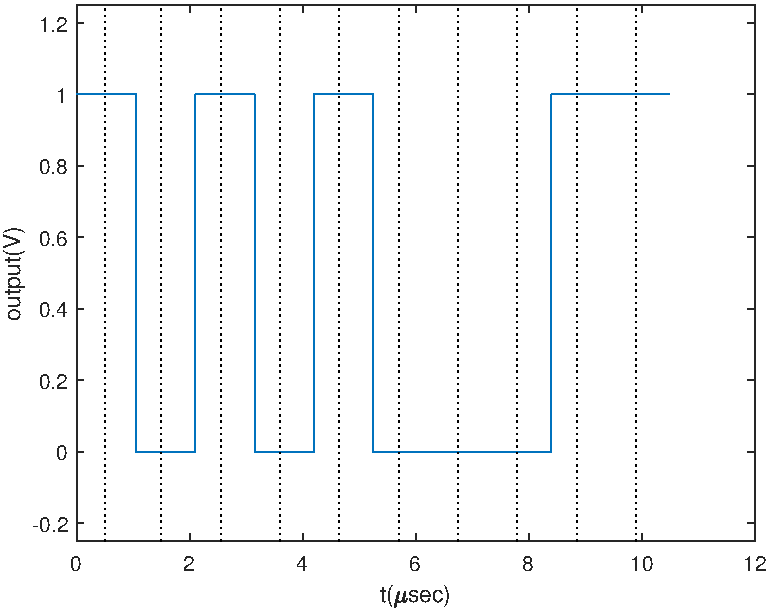
\includegraphics[width=2.5in]{problem3c.pdf}
    \end{center}
\end{figure}

\paragraph{d)}

Lets assume this noise causes the receiver to register a transition. Then at \(0.4\mu\)s the lag will be set to \(0.4\mu\)s. The first
sample will remain at \(0.5\mu\)s. At this time the predicted next transition will be at \(1.4\mu\)s. Then at the transition at \(1.05\mu\)s, the lag will be set to
\(-0.35\mu\)s. The next sampling will be at \(1.9\mu\)s. The predicted next transition will be at \(2.05\mu\)s. At \(2.10\mu\)s, the lag will be set to \(0.05\mu\)s.
The next sampling will be at \(2.55\mu\)s. From here on out the sequence of samples remains the same as in the previous part, leading to the sampling
happening at times \(0.5\mu\)s, \(1.9\mu\)s, \(2.55\mu\)s, \(3.60\mu\)s, \(4.65\mu\)s, \(5.70\mu\)s, \(6.75\mu\)s, \(7.80\mu\)s, \(8.85\mu\)s, and \(9.90\mu\)s.

\paragraph{e)}

Lets assume this noise causes the receiver to register a transition. The sampling will proceed normally until \(2.4\mu\)s. At \(2.4\mu\)s the receiver has a predicted
transition value of \(2.05\mu\)s, so it will calculate a lag of \(0.35\mu\)s. It will sample at \(2.55\mu\)s, updating the predicted transition value to \(3.4\mu\)s. At \(3.15\mu\)s,
the lag will be set to \(-0.25\mu\)s. A sample occurs at \(3.9\mu\)s, and the receiver updates the predicted transition value to \(4.15\mu\)s. At \(4.20\mu\)s, the lag is updated to
\(0.05\mu\)s. The next sample occurs at \(4.65\mu\)s. From here on out the sequence of samples remains the same as the previous part, leading to the sampling happening at times
 \(0.5\mu\)s, \(1.5\mu\)s, \(2.55\mu\)s, \(3.90\mu\)s, \(4.65\mu\)s, \(5.70\mu\)s, \(6.75\mu\)s, \(7.80\mu\)s, \(8.85\mu\)s, and \(9.90\mu\)s.

\section*{Problem 4}

\paragraph{a)}

You can send three bits every microsecond by having \(8\)V correspond to \(111\), \(6\)V correspond to \(110\), \(4\)V correspond to \(101\), \(2\)V correspond to \(100\),
\(-2\)V correspond to \(011\), \(-4\)V correspond to \(010\), \(-6\)V correspond to \(001\), and \(-8\)V correspond to \(000\).

\paragraph{b)}

No this coding scheme does not guarantee transitions, for example if all \(1\)'s were sent then the signal would stay at \(8\)V and if all \(0\)'s were sent then the signal would stay at \(-8\)V.

\paragraph{c)}

No this coding scheme is not DC balanced, as the signal could be a constant \(8\)V if all \(1\)'s are being sent.

\paragraph{d)}

The best DC balanced code I can think of is encoding \(11\) as either \(-8\)V or \(8\)V, \(10\) as either \(-6\)V or \(6\)V, \(01\) as either \(-4\)V or \(4\)V, and \(00\) as either \(-2\)V or \(2\)V.
The encoded signal would choose the appropriate inverse value for each bit sequence in order to make the signal DC balanced.

\paragraph{e)}

In this DC balanced code, two bits are transmitted each microsecond.

\paragraph{f)}

Yes, transitions can be guaranteed. This is because if a sequence of the same bit pattern is sent, we can simply send a voltage that is opposite in sign but the same magnitude. This way between any two
pairs of bit patterns there can be a transition.

\paragraph{g)}

The maximum amount of noise that this scheme can tolerate is noise with a magnitude of \(0.5\)V, due to the Shannon limit.

\section*{Problem 5}

We can send one bit every \(40\)ns without interference due to dispersion. This means that the maximum bit rate that we can use without causing intersymbol
interference is \(2.5\times 10^7\) bits per second. If we double the length of the fiber link, we can expect the difference between the longest route and shortest
route to increase to \(80\)ns. This will halve our bit rate to \(1.25\times 10^7\) bits per second.

\end{document}